\chapter{Campi locali}
In Meccanica classica che descrive il punto materiale, un sistema è descritto da un set di coordinate generalizzate $\{q_i\}$ e dalla lagrangiana $L(q_i,\dot{q}_i)$ che dipende dalle $q_i$ e dalle rispettive velocità generalizzate $\dot{q}_i$. Dal principio di minima azione $\delta S = 0$, dove $S = \int_{t}L(q_i,\dot{q}_i)\,dt$ è l'azione, si possono derivare le equazioni del moto di Eulero-Lagrange. In una teoria di campo ruolo delle coordinate $q_i$ è assunto proprio dal campo $\phi(\vx,t)$ in cui l'indice $i$ delle $q_i$ viene rimpiazzato da $\vx$ che varia con continuità. Come già accennato, la posizione non è un operatore come in Meccanica quantistica ma un parametro al pari del tempo $t$, entrambi aventi il ruolo di ``etichettare'' il campo $\phi(\vx,t)$ che si estende su un numero infinito di valori delle coordinate. Tuttavia, in una teoria di campo si prevede che possano coesistere campi diversi in uno stesso punto dello spazio, per cui si usa un indice aggiuntivo $\phi_i(\vx,t)$ per distinguerli. I campi vengono poi associati ad una lagrangiana che ne determina l'evoluzione temporale. Le teorie di campo che si trattano sono teorie locali, in cui la dinamica del sistema non collega punti diversi dello spazio istantaneamente, rispettando quindi il principio della Relatività speciale e la causalità degli eventi. Nelle teorie locali, i campi in qualsiasi regione dello spazio $R$ comunicano con lo spazio esterno ad $R$ solo attraverso i loro comportamento sulla superficie $\sigma$ di $R$. 
\begin{figure}[h]
    \centering
    \begin{tikzpicture}[scale=0.7]
        % Assi
        \draw[->] (0,0) -- (8,0) node[right] {$t$};
        \draw[->] (0,0) -- (0,4) node[above] {$x$};
        % Livelli x1 e x2
        \draw[dashed] (0,1) -- (2,1);
        \draw[dashed] (0,3) -- (2,3);
        \node[left] at (0,1) {$x_1$};
        \node[left] at (0,3) {$x_2$};
        % Tempi t1 e t2
        \draw[dashed] (2,0) -- (2,1);
        \draw[dashed] (7,0) -- (7,1);
        \node[below] at (2,0) {$t_1$};
        \node[below] at (7,0) {$t_2$};
        % Rettangolo R
        \draw (2,1) rectangle (7,3);
        \node at (4.5,2) {$R$};
        % Etichette P2
        \node[left] at (2,3.3) {$P_2$};
        \node[left] at (2,1.3) {$P_1$};
        % Etichetta theta
        \node[above] at (7,3) {$\sigma$};
    \end{tikzpicture}
    \caption{evoluzione temporale del sistema da $t_1$ a $t_2$.}
    \label{fig: evoluzione temporale}
\end{figure}
Quindi, in riferimento alla figura \ref{fig: evoluzione temporale}, per specificare i campi in ogni punto dello spaziotempo all'interno di $R$ è sufficiente specificare il valore dei campi in ogni punto interno ad $R$ negli istanti $t_1$ e $t_2$, e il valore dei campi in ogni punto sulla superficie $\sigma$ in tutti gli istanti di tempo $t$ compresi tra $t_1$ e $t_1$. Date queste condizioni, la lagrangiana ed il principio di minima azione descrivono l'evoluzione temporale dei campi per ogni istante $t_1 < t < t_2$ all'interno di $R$ tramite le equazioni del moto. 

\section{Dalla prima alla seconda quantizzazione}
Il processo di trattare le coordinate $q_i$ e $p_i$ in meccanica lagrangiana ed hamiltoniana è chiamata ``prima quantizzazione'', tuttavia nelle teorie di campo si studiano oggetti che hanno un numero infinito di gradi di libertà. La transizione tra Meccanica quantistica e Teoria dei campi avviene proprio passando dai tre gradi di libertà delle coordinate $x^i$ agli infiniti descritti dai campi $\phi(x^i)$ ed applicando direttamente ad essi i criteri di quantizzazione. 
\begin{figure}[h]
    \centering
    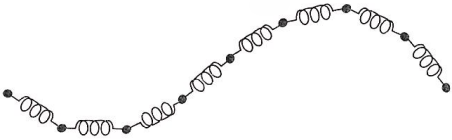
\includegraphics[width=0.5\linewidth]{Immagini/oscillatori armonici.png}
    \caption{sistema di infinite masse collegate da altrettante molle.}
    \label{fig: oscillatori armonici}
\end{figure}

Prima di effettuare questa transizione si può discutere come si descrivono in Meccanica classica sistemi con un numero infinito di gradi di libertà. A tal proposito, si consideri un numero $N$ masse collegate tra di loro da molle di costante elastica $k$, come mostrato in figura \ref{fig: oscillatori armonici}. La lagrangiana di questo sistema contiene due termini, l'energia potenziale di ogni molla e l'energia cinetica di ogni massa. Per cui, la lagrangiana è
\begin{equation}
    L = \sum_{i = 1}^{N}\frac{1}{2}\bigg[m_i\dot{x}_i^2 - k(x_i - x_{i+1})^2\bigg].
\end{equation}
Ora si supponga che si abbia un numero infinito di masse, $N\to\infty$, separate da una distanza $\epsilon$, per cui 
\begin{equation}
    L = \sum_{i = 1}^{N}\frac{\epsilon}{2}\bigg[\frac{m_i}{\epsilon}\dot{x}_i^2 - \frac{k}{\epsilon}(x_i - x_{i+1})^2\bigg],
\end{equation}
nel limite $\epsilon\to0$, la lagrangiana diventa
\begin{equation}
    L = \int\frac{1}{2}\bigg[\mu\dot{\phi}(x)^2 - Y\bigg(\frac{\p\phi(x)}{\p x}\bigg)^2\bigg]\,dx,
\end{equation}
dove $\mu = m/\epsilon$ è la densità di massa lineare, $Y = k\epsilon$ è il modulo di Young e dove si sono operate le estensioni al continuo
\begin{equation}
    \epsilon \to dx,\quad x_i \to \phi(x,t),
\end{equation}
indicando con $\phi(x,t)$ lo spostamento della singola particella localizzata nella posizione $x$ all'istante $t$. Usando le equazioni di Eulero-Lagrange per trovare le equazioni del moto si ritrova l'equazione delle onde unidimensionale 
\begin{equation}
    \frac{\p^2\phi}{\p x^2} - \frac{\mu}{Y}\frac{\p^2\phi}{\p t^2} = 0
\end{equation}
di un sistema che viaggia alla velocità $v = \sqrt{Y/\mu}$. Con questo, da una parte si è dimostrato il fatto che le onde possono propagarsi lungo una molla infinita, mentre dall'altra si è effettuata una transizione ad un sistema con infiniti gradi di libertà tutt'altro che banale. Questa generalizzazione si può vedere come il passaggio dalla lagrangiana $L(q_i,\dot{q}_i)$ ad una lagrangiana funzione dei campi e delle sue derivate spaziotemporali
\begin{equation}
    L(\phi(x^\mu),\p_\mu\phi(x^\mu)),
\end{equation}
definendo quindi l'azione $S$ come l'integrale in quattro dimensioni di una densità di lagrangiana $\mathcal{L}$
\begin{equation}
\label{eq: azione}
    S = \int\mathcal{L}\,d^4x = \int L\,dt,\quad L = \int\mathcal{L}(\phi,\p_\mu\phi)\,d^3x.
\end{equation}

\section{Trasformazioni di Poincarè}
Si consideri una funzione $f$ dipendente dalle coordinate spaziotemporali di un punto $P$. In un certo sistema di riferimento il punto $P$ ha coordinate $x^\mu$ e la funzione ha la forma $f(x^\mu)$, mentre in un altro ha coordinate $x'^\mu$, per cui la funzione è $f'(x'^\mu)$. Per un trasformazione infinitesima $x'^\mu = x^\mu + \delta x^\mu$, la variazione totale su $f$ è
\begin{equation}
    \begin{split}
        \Delta f &= f'(x'^\mu) - f(x^\mu) = f'(x^\mu + \delta x^\mu) - f(x^\mu) \\
        &= f'(x^\mu) - f(x^\mu) +\p_\mu f'(x^\mu)\delta x^\mu + O[(\delta x^\mu)^2].
    \end{split} 
\end{equation}
All'ordine più basso si può approssimare $\p_\mu f \simeq \p_\mu f'$, per cui
\begin{equation}
    \Delta f = \delta f +\p_\mu f\delta x^\mu,
\end{equation}
dove $\delta f$ è la variazione di $f$ dovuta al cambiamento della forma funzionale di $f$ e il secondo termine a secondo membro prende il nome di ``termine di trasporto''. Quindi, riassumendo, la variazione totale $\Delta$ è data dalla somma della variazione della forma funzionale $f$ e della variazione di $f$ indotta dalla variazione delle coordinate $\delta x^\mu\p_\mu$.

\subsubsection{Campo scalare}
Per definizione, un campo scalare è invariante sotto trasformazioni di Lorentz, ossia una funzione delle coordinate $x^\mu$ che assume lo stesso valore in tutti i sistemi di riferimento legati tra loro da una trasformazione di Lorentz, per cui $\phi(x^\mu) = \phi'(x'^\mu)$ e
\begin{equation}
    \Delta \phi = \delta\phi + \delta x^\mu\p_\mu\phi = 0.
\end{equation}
Considerando una traslazione infinitesima $x'^\mu = x^\mu + \epsilon^\mu$, con $\epsilon^\mu = \delta x^\mu$, si ha
\begin{equation}
    \Delta \phi = \delta \phi + \epsilon^\mu\p_\mu\phi = 0\quad\Rightarrow\quad\delta\phi = -\epsilon^\mu\p_\mu\phi = -i\epsilon^\mu p_\mu\phi,
\end{equation}
dove si è usata la definizione del quadrimpulso $p_\mu = -i\p_\mu$. Si deduce quindi che una traslazione spaziotemporale delle coordinate $x^\mu$ induce sul campo scalare una trasformazione generata dall'operatore impulso $p_\mu$. Per una traslazione finita si ha
\begin{equation}
    \phi' = (\MI - i\epsilon^\mu\p_\mu)\phi\quad\Rightarrow\quad \phi' = e^{-i\epsilon^\mu p _\mu}\phi.
\end{equation}
Considerando invece una traslazione di Lorentz spaziotemporale $x'^\mu = x^\mu + \delta x^\mu$, con $ \epsilon^{\mu\rho}x_\rho = \delta x^\mu$, si ha
\begin{equation}
    \Delta \phi = \delta \phi + \epsilon^{\mu\rho}x_\rho\p_\mu\phi = 0\quad\Rightarrow\quad\delta\phi = -\epsilon^{\mu\rho}x_\rho\p_\mu\phi.
\end{equation}
In questo caso l'identificazione del generatore con cui identificare l'operatore differenziale che agisce sul campo scalare non è così ovvia, antisimmetrizzando $\delta = -\epsilon^{\mu\rho}x_\rho\p_\mu$ si ottiene 
\begin{equation}
    \delta = -\frac{1}{2}\epsilon^{\mu\rho}(x_\rho\p_\mu - x_\mu\p_\rho) = -\frac{i}{2}\epsilon^{\mu\rho}M_{\rho\mu},
\end{equation}
dove $M_{\rho\mu}$ sono proprio i generatori delle trasformazioni di Lorentz in rappresentazione infinita. Quindi, per trasformazioni di Lorentz infinitesime si può scrivere
\begin{equation}
    \delta\phi = -\frac{i}{2}\epsilon^{\mu\rho}M_{\mu\rho}\phi,
\end{equation}
dove $M_{\mu\rho}$ sono operatori differenziali in cui indici sono opportunamente contratti con i parametri $\epsilon^{\mu\rho}$ per formare un operatore globalmente scalare sotto trasformazioni di Lorentz, ovviamente contengono al loro interno gli operatori di momento angolare e i generatori dei boost. Per una trasformazione finita si ha
\begin{equation}
    \phi' = e^{-i\epsilon^{\mu\rho}M_{\mu\rho}/2}\phi.
\end{equation}
Dunque, si conclude che una trasformazione di Lorentz sulle coordinate $x^\mu$ induce sul campo scalare una trasformazione generata dai generatori $M_{\mu\rho}$ delle trasformazioni di Lorentz.
\begin{obs}
    Nel caso particolare della rappresentazione scalare, all'interno di $M_{\mu\rho}$ non sono presenti gli operatori di momento di spin, ma solo quelli di momento angolare orbitale, proprio perché la rappresentazione scalare coincide con $\bm{(0,0)}$ che descrive una particella a spin zero.
\end{obs}
\begin{obs}
    Si possono generare molteplici tipi di campi scalari a partire da $\phi$ come $\phi^n$, $\cos{\phi}$, $\sin{\phi}$, $\p_\mu\p^\mu\phi$ e $\p_\mu\phi\p^\mu\phi$. Si deve però fare attenzione, ad esempio la combinazione $x^\mu\p_\mu\phi$ è un invariante di Lorentz, ma non è invariante per trasformazioni di Poincarè in quanto la derivata non distingue le traslazioni. 
\end{obs}

\subsubsection{Campo vettoriale}
Il campo vettoriale più semplice da costruire a partire dal campo scalare $\phi$ è $\p_\mu\phi$. Considerando una trasformazione infinitesima, la variazione di $\p_\mu\phi$ è data da
\begin{equation}
\label{eq: variazione campo vettoriale D_mu phi}
    \Delta(\p_\mu\phi) = \delta\p_\mu\phi + \delta x^\rho\p_\rho\p_\mu\phi,
\end{equation}
questa si può anche scrivere come
\begin{equation}
    \Delta(\p_\mu\phi) = \comm{\Delta}{\p_\mu}\phi + \p_\mu(\Delta\phi) = \comm{\Delta}{\p_\mu}\phi,
\end{equation}
dove si è usata l'ipotesi che il campo è scalare e quindi $\Delta\phi = 0$. Ora il commutatore ottenuto, considerando una trasformazione di Lorentz infinitesima, vale
\begin{equation}
    \comm{\Delta}{\p_\mu} = \comm{\delta x^\nu\p_\nu}{\p_\mu} = \comm{\epsilon^{\nu\rho}x_\rho\p_\nu}{\p_\mu},
\end{equation}
applicando il risultato a $\phi$ si ottiene
\begin{equation}
    \begin{split}
        \Delta(\p_\mu\phi) &=  \comm{\epsilon^{\nu\rho}x_\rho\p_\nu}{\p_\mu}\phi \\
        &= \epsilon^{\nu\rho}x_\rho\p_\nu(\p_\mu\phi) - \epsilon^{\nu\rho}\p_\mu(x_\rho\p_\nu\phi) \\
        &= \epsilon^{\nu\rho}x_\rho\p_\nu(\p_\mu\phi) - \epsilon^{\nu\rho}(\p_\mu x_\rho)(\p_\nu\phi) - \epsilon^{\nu\rho}x_\rho(\p_\mu\p_\nu\phi) \\
        &= - \epsilon^{\nu\rho}g_{\mu\rho}(\p_\nu\phi) \\
        &= \epsilon^\nu_\mu\p_\nu\phi,
    \end{split}
\end{equation}
dove si è usato il fatto che il prodotto tra $\epsilon^{\nu\rho}$, completamente antisimmetrico, e $\p_\nu\p_\nu$, completamente simmetrico, è nullo. Ora confrontando il risultato ottenuto con la \eqref{eq: variazione campo vettoriale D_mu phi} segue che
\begin{equation}
    \begin{split}
        \delta(\p_\mu\phi) &= \epsilon^\nu_\mu(\p_\nu\phi) - \epsilon^{\rho\sigma}x_\sigma\p_\rho(\p_\mu\phi) \\
        &= \epsilon^{\rho\sigma}g_{\rho\mu}g^\nu_\sigma(\p_\nu\phi) - \epsilon^{\rho\sigma}x_\sigma\p_\rho(\p_\mu\phi) \\
        &= \frac{1}{2}\epsilon^{\rho\sigma}[(g_{\rho\mu}g^\nu_\sigma - g_{\sigma\mu}g^\nu_\rho)(\p_\nu\phi) - (x_\sigma\p_\rho - x_\rho\p_\sigma)(\p_\mu\phi)] \\
        &=-\frac{i}{2}\epsilon^{\rho\sigma}(S_{\rho\sigma})^\nu_\mu(\p_\nu\phi) - \frac{i}{2}\epsilon^{\rho\sigma}L_{\rho\sigma}(\p_\mu\phi),
    \end{split}
\end{equation}
dove i $L_{\rho\sigma} = i(x_\sigma\p_\rho - x_\rho\p_\sigma)$ sono i generatori che racchiudono i momenti angolari orbitali ed i boost nello spaziotempo, mentre gli $(S_{\rho\sigma})^\nu_\mu = i(g_{\rho\mu}g^\nu_\sigma - g_{\sigma\mu}g^\nu_\rho)$ sono i generatori che contengono i momenti di spin, indipendenti dalle coordinate $x^\mu$ e dagli operatori di derivazione $\p^\mu$, soddisfacenti la stessa algebra dei momenti angolari. 

\subsubsection{Campo spinoriale}
Le rappresentazioni spinoriali del gruppo di Lorentz $\bm{(1/2,0)}$ e $\bm{(0,1/2)}$ sono realizzate attraverso i rispettivi spinori che si indicano con $\psi_L$ e $\psi_R$. Le proprietà di trasformazione sono
\begin{align}
    \psi_L(x^\mu) &\to \psi_L'(x'^\mu) = \ML_L\psi_L(x^\mu), \\
    \psi_R(x^\mu) &\to \psi_R'(x'^\mu) = \ML_R\psi_R(x^\mu),
\end{align}
con $\ML_{L,R}\in\mathbb{C}^{2,2}$. Quando la trasformazione è una rotazione, si sa dalla rappresentazione spinoriale di $SU(2)$ che
\begin{equation}
    \ML_L^{(r)} = \ML_R^{(r)} = e^{i\sigma_i\omega^i/2},
\end{equation}
dove le matrici di Pauli $\sigma^i$ soddisfano la relazione $\sigma^i\sigma^j = \delta^{ij} + i\epsilon^{ijk}\sigma_k$. Invece, se la trasformazione è una boost, dalla medesima rappresentazione si sa che
\begin{equation}
    \ML^{(b)}_L = e^{-\sigma_i\eta^i/2},\quad\ML_R^{(b)} = e^{\sigma_i\eta^i/2}.
\end{equation}
Quindi, per una trasformazione di Lorentz
\begin{equation}
    \begin{cases}
        \ML_L = e^{i\sigma_i(\omega^i - i\eta^i)/2} \\
        \ML_R = e^{i\sigma_i(\omega^i + i\eta^i)/2}
    \end{cases},
\end{equation}
dove le matrici $\ML$ soddisfano le seguenti proprietà
\begin{equation}
    \ML_L^{-1} = \ML_R^\dagger,\quad\sigma^2\ML_L\sigma^2 = \ML_R^*,\quad\ML_{L,R}^T = \sigma^2\ML_{L,R}^{-1}\sigma^2,\quad\ML_L^T\sigma^2\ML_L = \sigma^2.
\end{equation}
Usando unicamente gli spinori sinistrorsi o quelli destrorsi non è possibile definire un invariante di Lorentz, ma dato che questi sono legati da una trasformazione di parità, gli invarianti possono essere solo costruiti combinando $\psi_L$ con $\psi_R$, cioè combinando le due rappresentazioni $\bm{(0,1/2)}$ e $\bm{(1/2,0)}$. Come già visto, il modo più semplice per farlo è costruire uno spinore di Dirac
\begin{equation}
    \psi = 
    \begin{pmatrix}
        \psi_L \\
        \psi_R
    \end{pmatrix},
\end{equation}
le cui proprietà di trasformazione di parità sono ben definite
\begin{equation}
    \psi= 
    \begin{pmatrix}
        \psi_L \\
        \psi_R
    \end{pmatrix}
    \xrightarrow{P} \psi^P = 
    \begin{pmatrix}
        \psi_R \\
        \psi_L
    \end{pmatrix} =
    \begin{pmatrix}
        \MO & \MI \\
        \MI & \MO
    \end{pmatrix}
    \begin{pmatrix}
        \psi_L \\
        \psi_R
    \end{pmatrix},
\end{equation}
dove si definisce la nuova matrice
\begin{equation}
    \gamma^0 := 
    \begin{pmatrix}
        \MO & \MI \\
        \MI & \MO
    \end{pmatrix}.
\end{equation}
In generale, si possono scrivere gli invarianti bilineari in funzione degli spinori di Dirac come
\begin{equation}
    \psi_R^\dagger\psi_L + \psi_L^\dagger\psi_R = \psi^\dagger\gamma^0\psi = \bar{\psi}\psi,\quad\bar{\psi} := \psi^\dagger\gamma^0,
\end{equation}
e
\begin{equation}
    \frac{1}{2}(\psi_L^\dagger\sigma^\mu\p_\mu\psi_L + \psi_R^\dagger\bar{\sigma}^\mu\p_\mu\psi_R) = \frac{1}{2}\bar{\psi}\gamma^\mu\p_\mu\psi,
\end{equation}
dove le matrici di Dirac $\gamma^\mu$ sono definite come
\begin{equation}
    \gamma^\mu := 
    \begin{pmatrix}
        \MO & \sigma^\mu \\
        \bar{\sigma}^\mu & \MO
    \end{pmatrix},\quad\sigma^\mu = (\MI,\sigma^i),\,\bar{\sigma}^\mu = (\MI,-\sigma^i),
\end{equation}
che rappresentano una sorta di estensione quadridimensionale delle matrici di Pauli. A partire dalle matrici di Dirac si può definire un'altra matrice $\gamma^5$ come
\begin{equation}
    \gamma^5 := i\gamma^0\gamma^1\gamma^2\gamma^3 = 
    \begin{pmatrix}
        -\MI & \MO \\
        \MO & \MI
    \end{pmatrix},
\end{equation}
con la quale è possibile definire gli operatori proiettori 
\begin{equation}
\label{eq: proiettori rappr. Dirac}
    \begin{cases}
        \hatP_{L} = \dfrac{1}{2}(\MI - \gamma^5) \\[2ex]
        \hatP_R = \dfrac{1}{2}(\MI + \gamma^5),
    \end{cases}
\end{equation}
i quali agiscono su $\psi$ in modo da ``selezionare'' solo una tra le componenti $\psi_L$ e $\psi_R$, ossia
\begin{equation}
    \hatP_L\psi = 
    \begin{pmatrix}
        \psi_L \\
        0
    \end{pmatrix},\quad
    \hatP_R\psi = 
    \begin{pmatrix}
        0 \\
        \psi_R
    \end{pmatrix}.
\end{equation}
Inoltre, le matrici di Dirac soddisfano le regole di anticommutazione dell'algebra di Clifford
\begin{equation}
\label{eq: algebra di Clifford}
    \acomm{\gamma^\mu}{\gamma^\nu} = 2g^{\mu\nu}.
\end{equation}
In particolare, la matrice di chiralità anticommuta con tutte le matrici di Dirac, per cui
\begin{equation}
    \acomm{\gamma^\mu}{\gamma^5} = 0.
\end{equation}






